\section{COVID-19 and Its Effect on Hospital Capacity} \label{sub: Hospital Capacity}

A region's hospital capacity is in direct correlation with survival rates for the region's citizens. Therefore, having a hospital capacity that can withstand COVID-19 is vital for a society's ability to likewise withstand the pandemic. 

Since COVID-19 spread across the globe in early spring of 2020, each country's hospital capacity has been tested. Director of the Danish Health Authority, Søren Brostrøm, published a statement in March 2020 regarding nationwide strain on hospital capacity and a plan moving forward \citep{brostrom_notat_2020}. In this statement, he urged patients to minimise hospital visits and also gave examples of which operations can be postponed until Danish hospitals can move safely past COVID-19.

Some scholars have simulated hospital capacity on local scales, such as Weissman et al., whose aim is to predict hospital capacity needs within the greater area of Philadelphia, Pennsylvania, USA \citep{weissman_locally_2020}. Unfortunately, and as mentioned by Weissman et al., parameters for these types of simulations are typically taken from published data from heterogeneous sources. As stated in section \vref{sub: Statistical Uncertainty} in this report, this is also a limitation that we have encountered throughout data collection for our simulation.

Our proposal for analysing COVID-19's effect on hospital capacity is instead to see hospital capacity as a static number and compare this static value to the number of severely infected in our source code (see Appendix \ref{Appendix: SourceCode} Source Code). From the get-go, we have viewed our severely infected medical state as the medical state needing medical care.

\subsection{Definition of Hospital Capacity}

What is meant with the phrase \say{hospital capacity}? Each hospital has some influence on what is meant with this phrase, meaning that there is not a universal definition. However, all hospitals within the same country have. Because the scope of this project's simulation is limited to the greater Aalborg area, we will use a Danish definition of hospital capacity. This definition includes the following for each hospital:
\begin{itemize}
\item Available medical personnel
\item Available beds for patients
\item Available beds for patients within the Intensive Care Unit (ICU)
\item Available respirators for patients
\end{itemize}

If a hospital is reaching its capacity, patients can be moved to other hospitals. Therefore, while the individual hospital has its own capacity, the phrase \say{hospital capacity} can also refer to the entire nation's capacity.

For this project and simulation, which is based on a much smaller geographical scale, we will focus on the hospital capacity of Aalborg.

\subsection{Hospital Capacity in Denmark}

The hospital capacity within Denmark has steadily risen since the beginning of the COVID-19 pandemic in preparation for an aggravated increase in infected people. Specifically for Aalborg and Northern Jutland, a pandemic unit was established with 47 beds in total; 30 regular beds and 17 beds for intensive care \citep{dansk_sygeplejerad_fra_2020}. The number of respirators for each hospital remains unknown, but this information gives us a number to calculate with.

An important note to add on to this is the fact that hospitals can adapt relatively quickly to an increase in patients. As seen on esundhed.dk, the number of occupied beds in ICUs (Intensive Care Units) in Aalborg hospitals increased dramatically during March and April (\cite{esundheddk_sengepladser_2020}). March and April were the months throughout which the pandemic was at its first peak. Precise numbers were 32 beds in February, 78.8 in March, 90.9 in April and 51.3 in May. 

 

\subsection{Our Simulation's Hospital Capacity Results}

As with all other figures in chapter \ref{chap:result}: Results, the graphs on hospitalisation are based on the 808420 seed. As can be seen in figure \vref{fig:hospitalized NO CT}, hospitalisation peaks just about the same time as peak of infection (as seen in figure \vref{Fig:covidInfGraphs}). Infection peaks around day 112, whereas hospitalisation peaks around day 108. Since hospitalisation is dependent upon severe infection, the correlation is logical. The peak for hospitalisation is 200 people.

\begin{figure}[H]
  \centering
  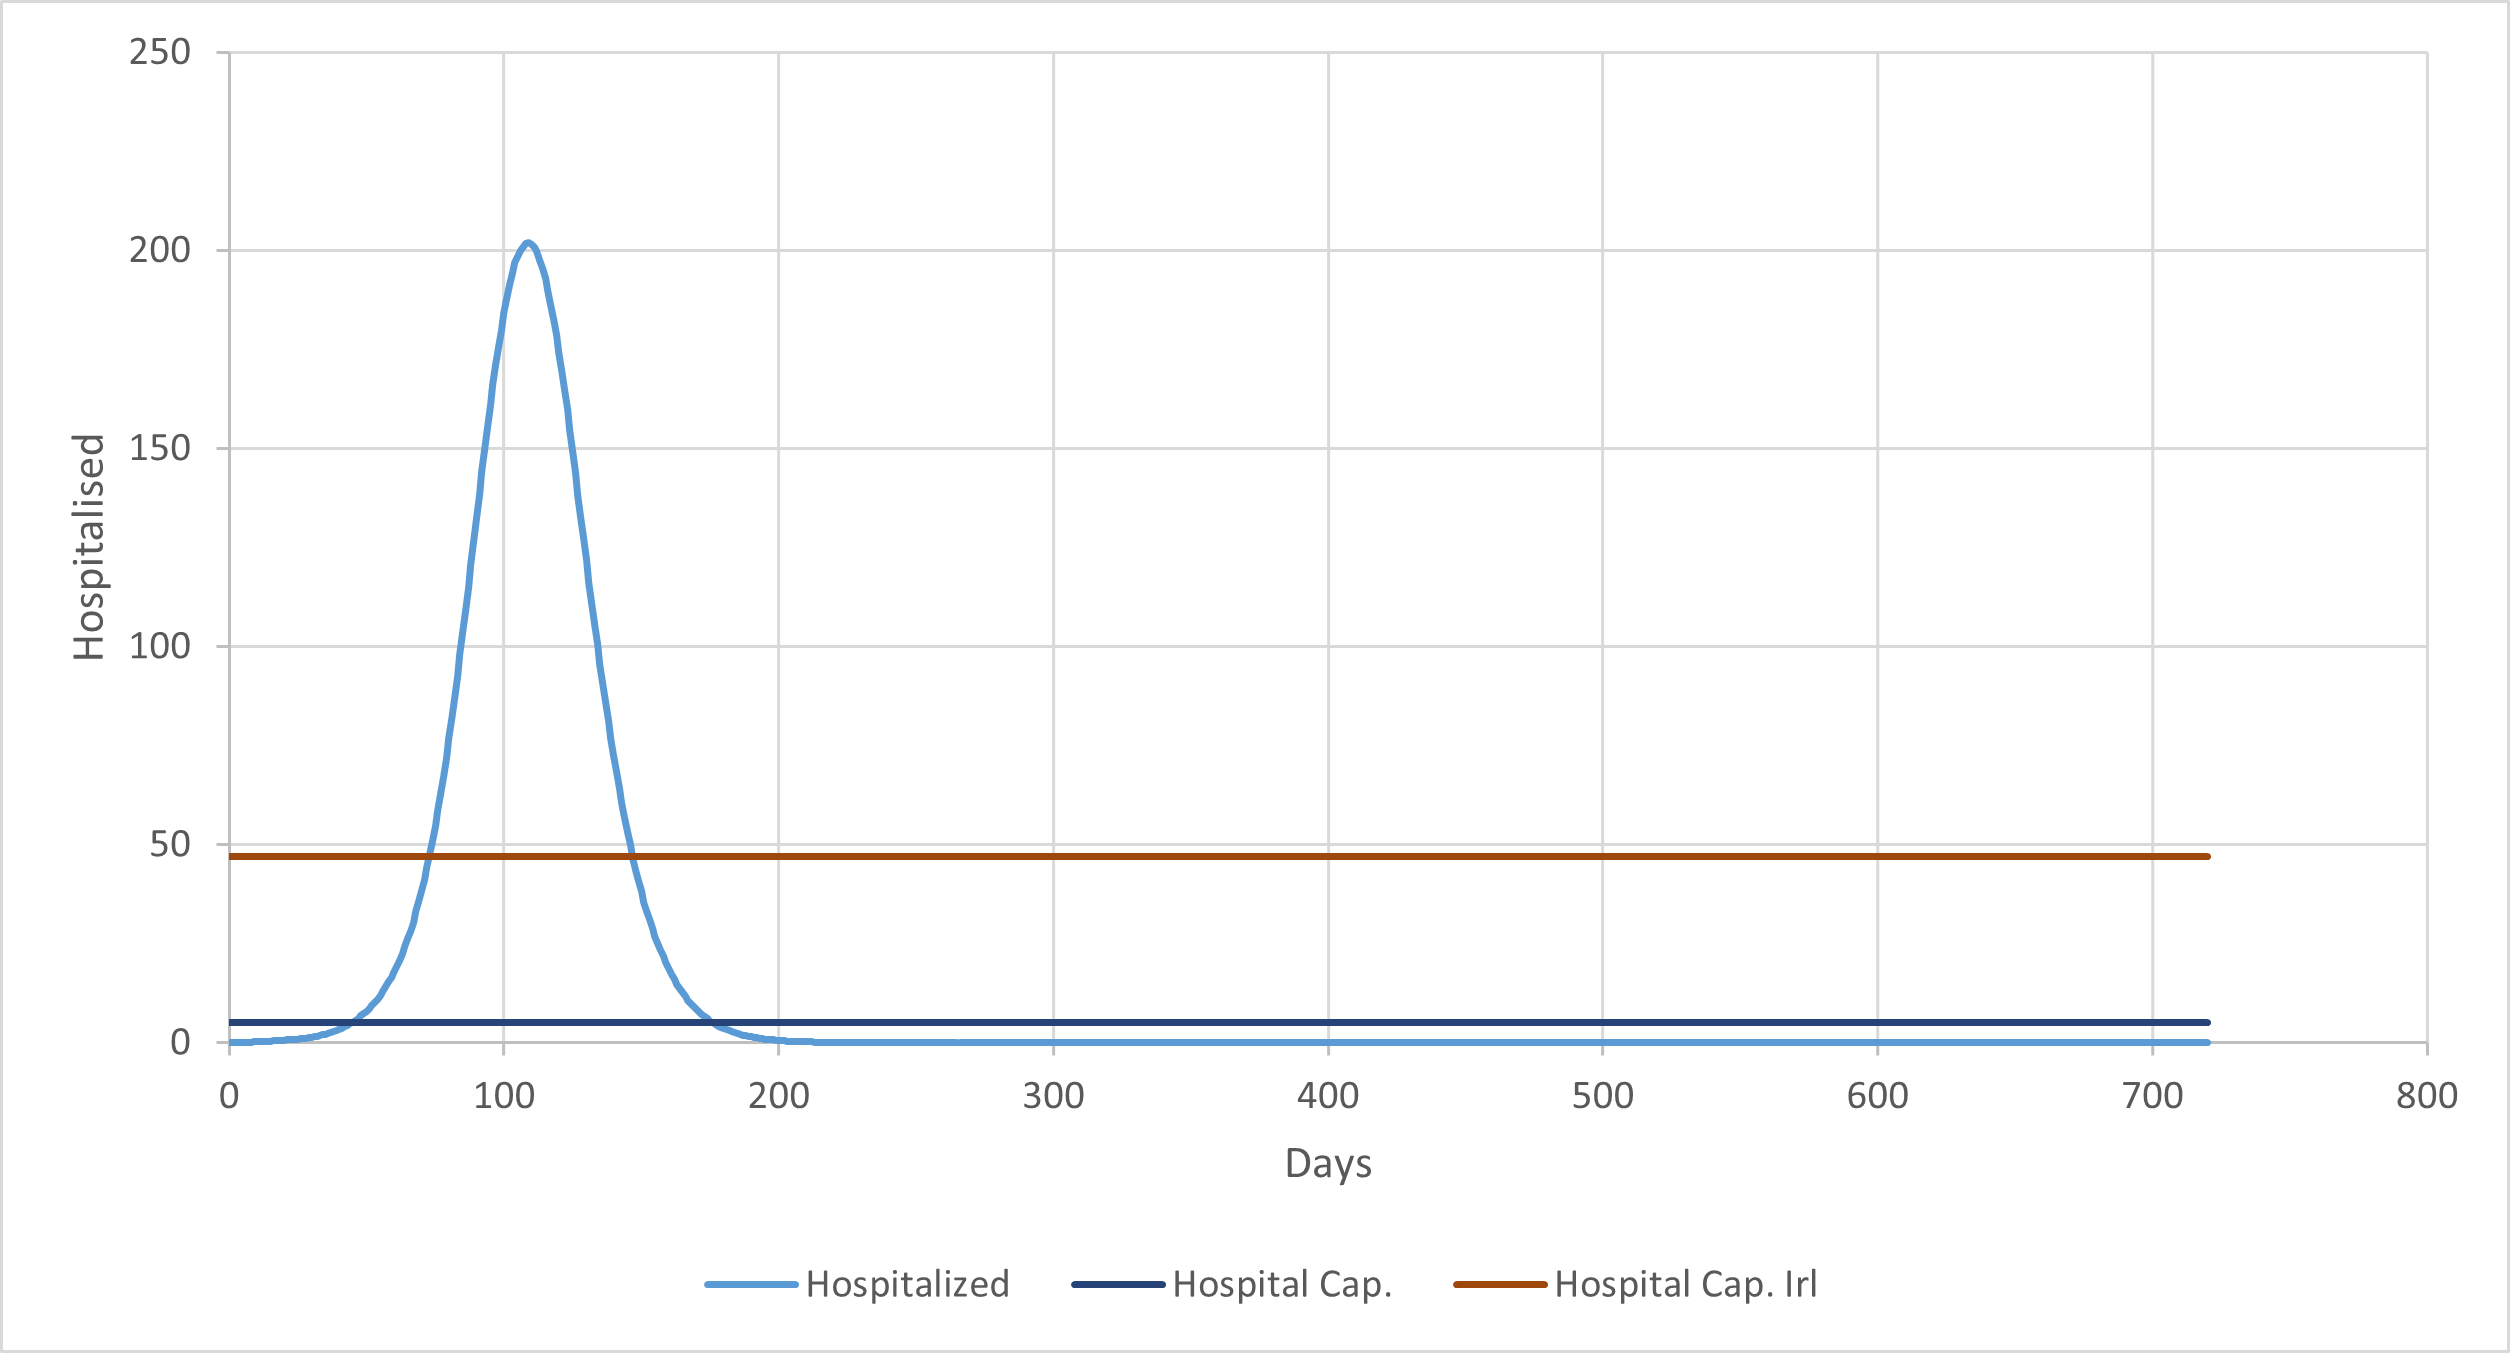
\includegraphics[width=140mm]{0_billeder/HOS_NO_CT.png}
  \caption{Hospitalised patients per day throughout the simulation with contact tracing disabled. Red line is regional hospital capacity, blue line is hospital capacity scaled to the sim population.}
  \label{fig:hospitalized NO CT}
\end{figure}
%Note tal for hospitals capacitet
As previously stated, the hospital capacity for our entire population (Aalborg area) is 47 beds in total. Therefore, the hospital capacity for our simulation is greatly exceeded. Whether our simulation is seen as representative for the entire population of Denmark or comparative to similar simulations for the rest of Denmark, it can be inferred that this excess in hospitalised patients can be disastrous. Even if taking into account that Aalborg Universitetshospital allowed for 90.9 patients during the highest peak of the pandemic's first wave, there is still an excess of more than 100 percent.

While the infection relatively quickly dies off again in this simulation (under the assumption that re-infection and mutation are not possible), the human and economic cost of exceeding hospital capacity by this much would be quite large.

In comparison, the figure for hospitalisations in a simulation where contact tracing is enabled is quite different, as seen below.

\begin{figure}[H]
  \centering
  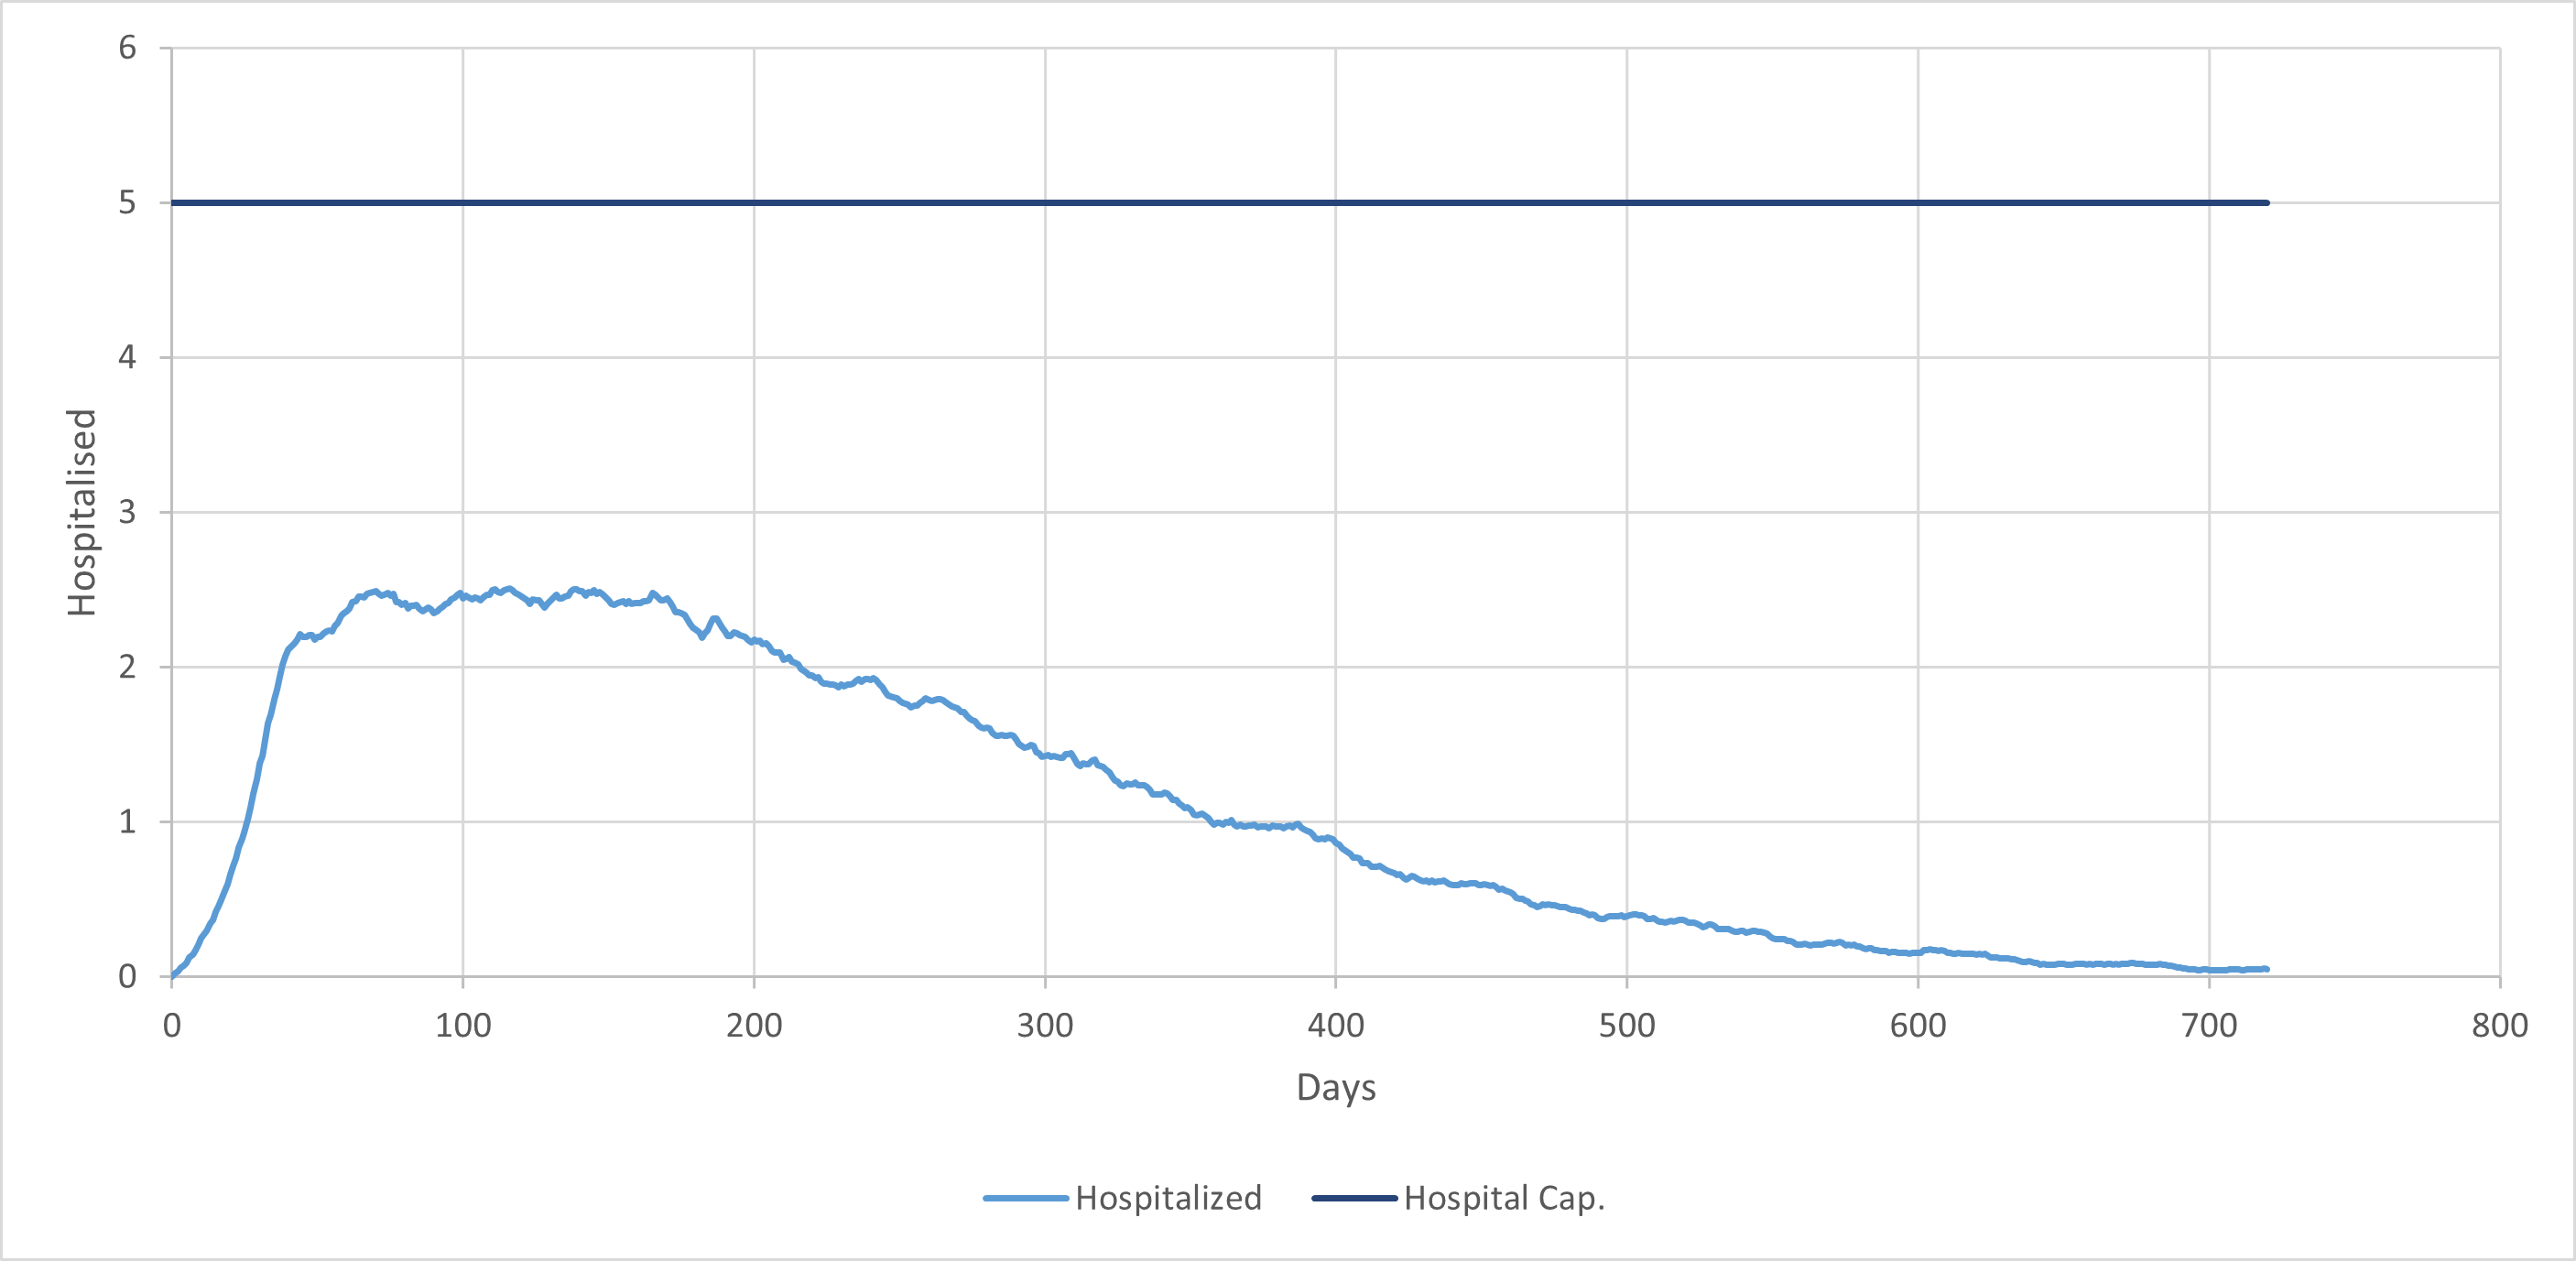
\includegraphics[width=140mm]{0_billeder/HOS_CT.png}
  \caption{Hospitalised patients per day throughout the simulation with contact tracing enabled. Blue line is hospital capacity scaled to the sim population.}
  \label{fig:hospitalized WITH CT}
\end{figure}

As seen in figure \vref{fig:hospitalized WITH CT}, it takes considerably longer for the hospitalisations to die out compared to figure \vref{fig:hospitalized NO CT}. However, the number of hospitalisations is a fraction of the hospitalisations for the simulation with no contact tracing. Therefore, while hospitals will have to deal with infected patients for much longer, the human and economic cost of a pandemic where contact tracing is implemented is dramatically reduced.

It should be noted here that figure \ref{fig:hospitalized WITH CT} is a graph of average hospitalisations with contact tracing enabled across all 1,000 drops in the simulation. Therefore, it is possible that some drops show a higher hospitalisation than others. See figure for all hospitalisations in each drop.

% Potentially insert histogram with hos.cap. included and make some observations here

As shown in figure \vref{fig:hospitalized WITH CT}, the number peaks around day 90 and maintains this peak for almost 100 days. However, the peak is at 2.5 hospitalisations. Therefore, the hospital capacity for the population in our simulation is not remotely exceeded.

There are naturally more factors to consider. Since Denmark makes use of pandemic units that are completely closed off from the outside world (\cite{dansk_sygeplejerad_fra_2020}), risk of further infecting other civilians as well as medical personnel is likewise reduced.